\vspace{-0.05in}
\section{Spatial Memory Network for VQA}\label{sec:smem}
\vspace{-0.05in}

%putting overview figure here to force it to appear on first Approach page
\begin{figure*}[t!]
\centering
%\includegraphics[width=.9\linewidth]{figures/overview_new.pdf}
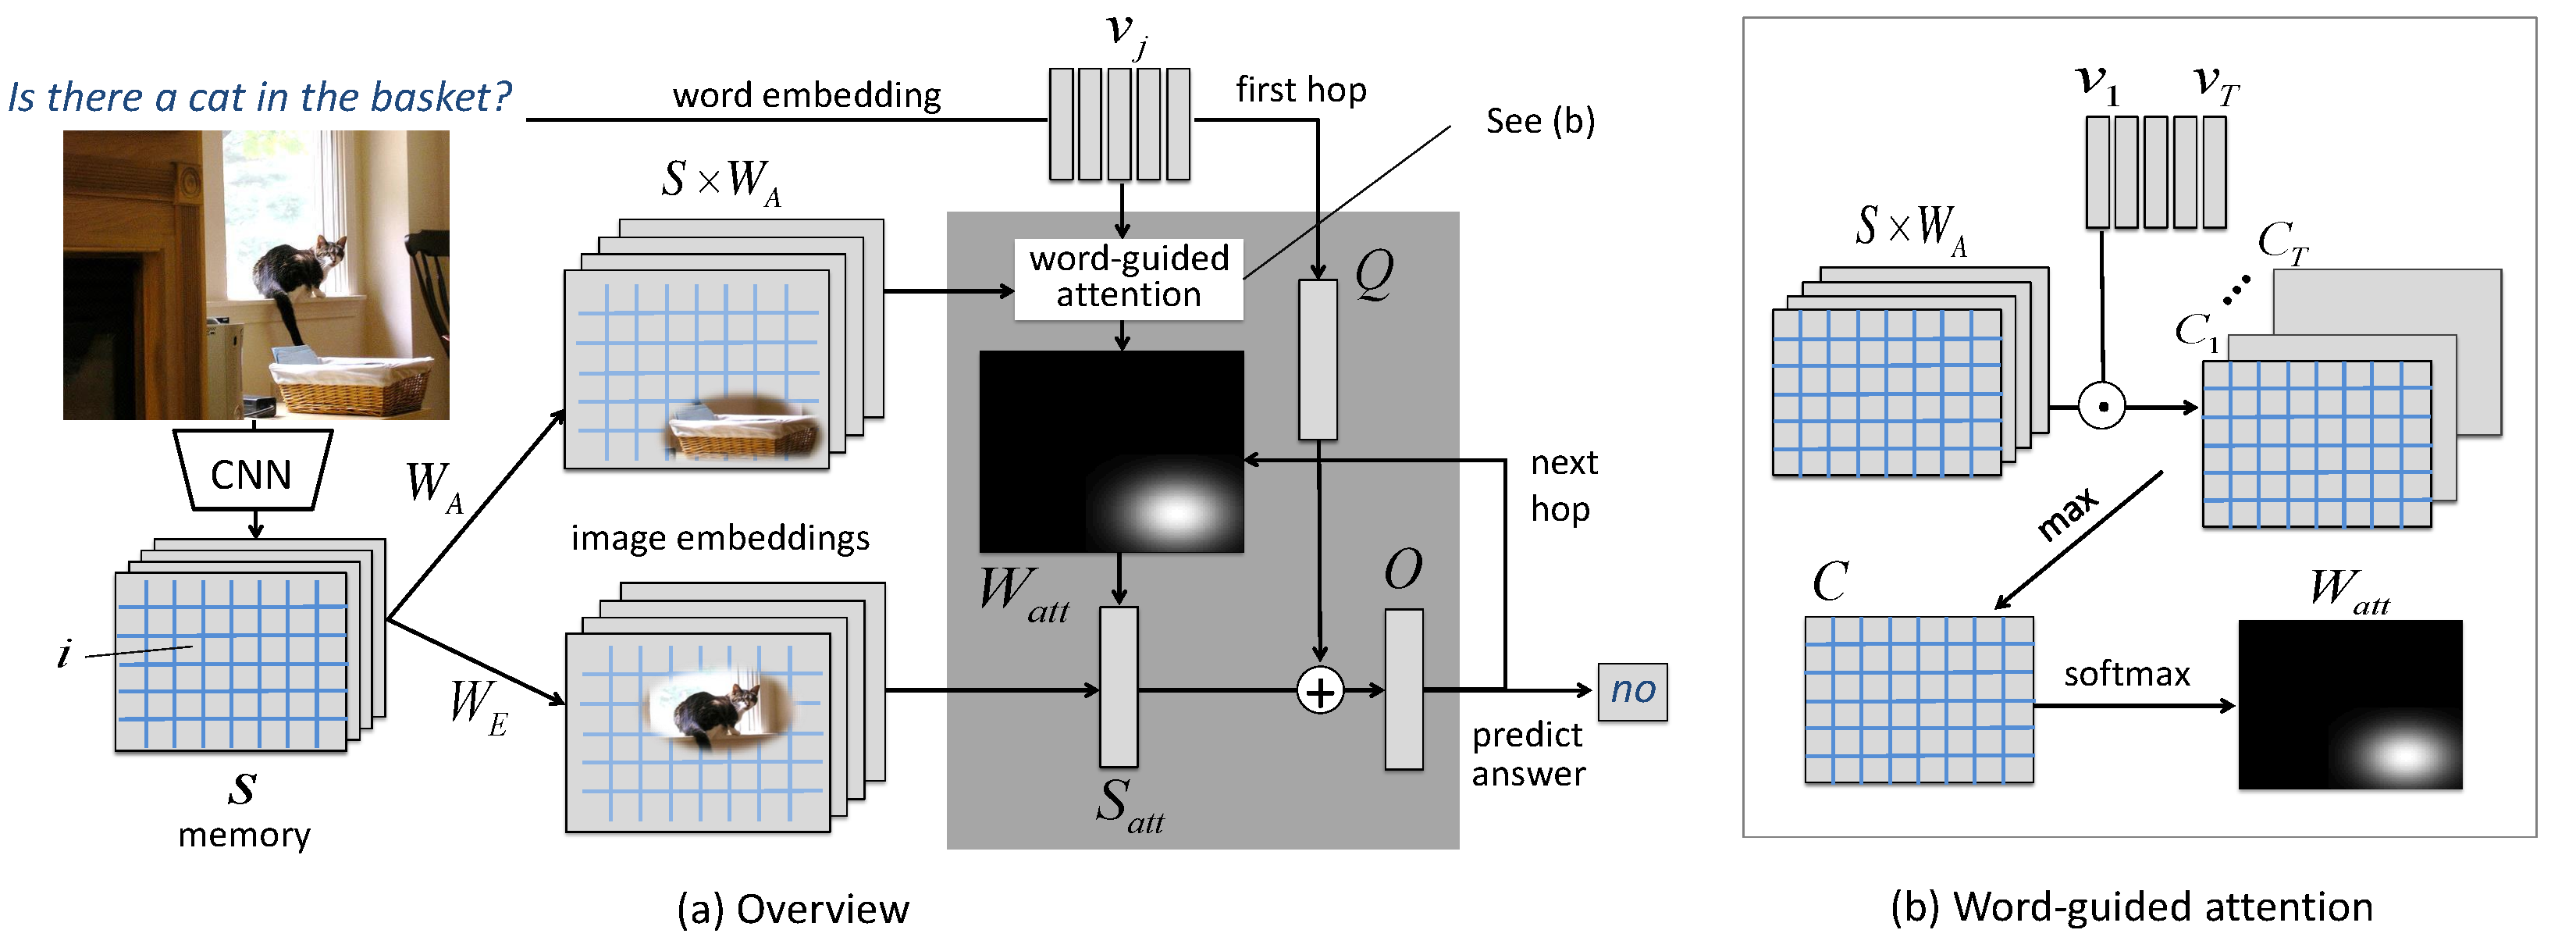
\includegraphics[width=.9\linewidth]{figures/overview_new2.pdf}
\vspace{-0.05in}
\caption{Our proposed Spatial Memory Network for Visual Question Answering (SMem-VQA). (a) Overview. First, the CNN activation vectors $S=\{s_i\}$ at image locations $i$ are projected into the semantic space of the question word vectors $v_j$ using the ``attention'' visual embedding $W_A$ (Sec.~\ref{sec:smem}). The results are then used to infer spatial attention weights $W_{att}$ using the word-guided attention process shown in (b). 
(b) Word-guided attention. This process predicts attention determined by the question word that has the maximum correlation with embedded visual features at each location, e.g. choosing the word \textit{basket} to attend to the location of the basket in the above image (Sec.~\ref{sec:att1}).
The resulting spatial attention weights $W_{att}$ are then used to compute a weighted sum over the visual features embedded via a separate ``evidence'' transformation $W_E$, e.g., selecting evidence for the cat concept at the basket location. Finally, the weighted evidence vector $S_{att}$ is combined with the full question embedding $Q$ to predict the answer. An additional hop can repeat the process to gather more evidence (Sec.~\ref{sec:att3}). 
}
\label{fig:illus}
\vspace{-0.15in}
\end{figure*}

%%%%%%%%%%%%%%%%%%%%%%%%%%%%%%%%%%%%%%%%%%%%%%%%%%%%%%%%%%%%%%%%%%%%%%%%%%%%%%%%%%%%%%%%%%%%%
%\subsection{Overview}
We first give an overview of the proposed SMem-VQA network, illustrated in Fig.~\ref{fig:illus} (a). Sec.~\ref{sec:att1} details the word-guided spatial attention process of the first hop shown in Fig.~\ref{fig:illus} (b), and Sec.~\ref{sec:att3} describes adding a second hop into SMem-VQA network.

The input to our network is a question comprised of a variable-length sequence of words, and an image of fixed size.
Each word in the question is first represented as a one-hot vector in the size of the vocabulary, with a value of one only in the corresponding word position and zeros in the other positions. Each one-hot vector is then embedded into a real-valued word vector, $V=\{v_j \;|\;v_j\in \mathbb{R}^N; j=1,\cdots,T\}$, where $T$ is the maximum number of words in the question and $N$ is the dimensionality of the embedding space. Sentences with length less than $T$ are padded with special \textbf{$-1$} value, which are embedded to all-zero word vector.

The words in questions are used to compute attention over the visual memory, which contains extracted image features. The input image is processed by a convolutional neural network (CNN) to extract high-level $M$-dimensional visual features on a grid of spatial locations. 
Specifically, we use $S=\{s_i \;|\;s_i\in \mathbb{R}^M; i=1,\cdots,L\}$ to represent the spatial CNN features at each of the $L$ grid locations. In this paper, the spatial feature outputs of the last convolutional layer of GoogLeNet ($inception\_5b/output$) \cite{googlenet} are used as the visual features for the image. 

The convolutional image feature vectors at each location are  embedded into a common semantic space with the word vectors.
Two different embeddings are used: the ``attention'' embedding $W_A$ and the ``evidence'' embedding $W_E$. 
The attention embedding projects each visual feature vector such that its combination with the embedded question words generates the attention weight at that location. The evidence embedding detects the presence of semantic concepts or objects, and the embedding results are multiplied with attention weights and summed over all locations to generate the visual evidence vector $S_{att}$. 

Finally, the visual evidence vector is combined with the question representation and used to predict the answer for the given image and question.
In the next section, we describe the one-hop Spatial Memory network model and the specific attention mechanism it uses in more detail. 

%%%%%%%%%%%%%%%%%%%%%%%%%%%%%%%%%%%%%%%%%%%%%%%%%%%%%%%%%%%%%%%%%%%%%%%%%%%%%%%%%%%%%%%%%%%%%
\subsection{Word Guided Spatial Attention in One-Hop Model}\label{sec:att1}
Rather than using the bag-of-words question representation to guide attention,
the attention architecture in the first hop (Fig.~\ref{fig:illus}(b)) uses each word vector separately to extract correlated visual features in memory. 
The intuition is that the BOW representation may be too coarse, and letting each word select a related region may provide more fine-grained attention. 
The correlation matrix $C \in \mathbb{R}^{T\times L}$ between word vectors $V$ and visual features $S$ is computed as
\begin{equation}
C = V \cdot (S \cdot W_A + b_A)^T
\end{equation}
where $W_A \in \mathbb{R}^{M\times N}$ contains the attention embedding weights of visual features $S$, and $b_A \in \mathbb{R}^{L\times N}$ is the bias term. 
This correlation matrix is the dot product result of each word embedding and each spatial location's visual feature, thus each value in correlation matrix $C$ measures the similarity between each word and each location's visual feature. 

The spatial attention weights $W_{att}$ are calculated by taking maximum over the word dimension $T$ for the correlation matrix $C$, selecting the highest correlation value for each spatial location, and then applying the softmax function
\begin{equation}
W_{att} = \softmax(\max_{i=1,\cdots,T}(C_i)), ~C_i \in \mathbb{R}^L
\end{equation}
The resulting attention weights $W_{att} \in \mathbb{R}^{L}$ are high for selected locations and low for other locations, with the sum of weights equal to $1$. For instance, in the example shown in Fig.~\ref{fig:illus}, the question ``Is there a cat in the basket?'' produces high attention weights for the location of the basket because of the high correlation of the word vector for \textit{basket} with the visual features at that location. 

The evidence embedding $W_E$ projects visual features $S$ to produce high activations for certain semantic concepts. E.g., in Fig.~\ref{fig:illus}, it has high activations in the region containing the cat. The results of this evidence embedding are then multiplied by the generated attention weights $W_{att}$, and summed to produce the selected visual ``evidence'' vector $S_{att} \in \mathbb{R}^N$,
\begin{equation}
S_{att} = W_{att} \cdot (S \cdot W_E + b_E) \label{eqn:evidence}
\end{equation}
where $W_E \in \mathbb{R}^{M\times N}$ are the evidence embedding weights of the visual features $S$, and $b_E \in \mathbb{R}^{L\times N}$ is the bias term.
In our running example, this step accumulates \textit{cat} presence features at the \textit{basket} location. 

Finally, the sum of this evidence vector $S_{att}$ and the question embedding $Q$ is used to predict the answer for the given image and question.
For the question representation $Q$, we choose the bag-of-words (BOW). Other question representations, such as an LSTM, can also be used, however, BOW has fewer parameters yet has shown good performance. As noted in~\cite{shih2015look}, the simple BOW model performs roughly as well if not better than the sequence-based LSTM for the VQA task. Specifically, we compute
\begin{equation}
Q = W_Q \cdot V + b_Q
\end{equation}
where $W_Q \in \mathbb{R}^T$ represents the BOW weights for word vectors $V$, and $b_Q \in \mathbb{R}^{N}$ is the bias term. The final prediction $P$ is
\begin{equation}
P = \softmax(W_P \cdot f(S_{att} + Q) + b_P)\label{eqn:predict}
\end{equation}
where $W_P \in \mathbb{R}^{K\times N}$, bias term $b_P \in \mathbb{R}^{K}$, and $K$ represents the number of possible prediction answers. $f$ is the activation function, and we use ReLU here.
In our running example, this step adds the evidence gathered for \textit{cat} near the basket location to the question, and, since the cat was not found, predicts the answer ``no''. 
The attention and evidence computation steps can be optionally repeated in another hop, before predicting the final answer, as detailed in the next section. 

%%%%%%%%%%%%%%%%%%%%%%%%%%%%%%%%%%%%%%%%%%%%%%%%%%%%%%%%%%%%%%%%%%%%%%%%%%%%%%%%%%%%%%%%%%%%%
\subsection{Spatial Attention in Two-Hop Model}\label{sec:att3}
We can repeat hops to promote deeper inference, gathering additional evidence at each hop. Recall that the visual evidence vector $S_{att}$ is added to the question representation $Q$ in the first hop to produce an updated question vector,
\begin{equation}{O_{hop1} = S_{att} + Q}\end{equation}
On the next hop, this vector $O_{hop1} \in \mathbb{R}^{N}$ is used in place of the individual word vectors $V$ to extract additional correlated visual features to the whole question from memory and update the visual evidence.

The correlation matrix $C$ in the first hop provides fine-grained local evidence from each word vectors $V$ in the question, while the correlation vector $C_{hop2}$ in next hop considers the global evidence from the whole question representation $Q$. 
The correlation vector $C_{hop2} \in \mathbb{R}^L$ in the second hop is calculated by 
\begin{equation}
C_{hop2} = (S \cdot W_E + b_E) \cdot O_{hop1}
\end{equation}
where $W_E \in \mathbb{R}^{M\times N}$ should be the attention embedding weights of visual features $S$ in the second hop and $b_E \in \mathbb{R}^{L\times N}$ should be the bias term. Since the attention embedding weights in the second hop are shared with the evidence embedding in the first hop, so we directly use $W_E$ and $b_E$ from first hop here. 

The attention weights in the second hop $W_{att2}$ are obtained by applying the softmax function to the correlation vector $C_{hop2}$.
\begin{equation}
W_{att2} = \softmax(C_{hop2})
\end{equation}

Then, the correlated visual information in the second hop $S_{att2} \in \mathbb{R}^N$ is extracted using attention weights $W_{att2}$.
\begin{equation}
S_{att2} = W_{att2} \cdot (S \cdot W_{E_2} + b_{E_2})
\end{equation}
where $W_{E_2} \in \mathbb{R}^{M\times N}$ are the evidence embedding weights of visual features $S$ in the second hop, and $b_{E_2} \in \mathbb{R}^{L\times N}$ is the bias term. 

The final answer $P$ is predicted by combining the whole question representation $Q$, the local visual evidence $S_{att}$ from each word vector in the first hop and the global visual evidence $S_{att2}$ from the whole question in the second hop,
\begin{equation}
P = \softmax(W_P \cdot f(O_{hop1} + S_{att2}) + b_P)
\end{equation}
where $W_P \in \mathbb{R}^{K\times N}$, bias term $b_P \in \mathbb{R}^{K}$, and $K$ represents the number of possible prediction answers. $f$ is activation function. More hops can be added in this manner. 

The entire network is differentiable and is trained using stochastic gradient descent via standard backpropagation, allowing image feature extraction, image embedding, word embedding and answer prediction to be  jointly optimized on the training image/question/answer triples. 